%\documentclass[10pt,a4paper]{book}
%\usepackage[utf8]{inputenc}
%\usepackage{amsmath}
%\usepackage{amsfonts}
%\usepackage{amssymb}
%\usepackage{graphicx} 
%
%
%\begin{document}
%En esta sección se describe la preparación del conjunto de datos, 
%la selección de la estructura y los parámetros del modelo de aprendizaje profundo.

\section{Descripción del servicio sobre CloudNAO}


\subsection{Descripción del conjunto de datos\label{sec:dataset-def}}

Son cuatro las categorías en las que se quiere
clasificar una imagen obtenida por el robot: el cubículo,
la salida de emergencia, la cancha de fútbol y la zona de trabajo.

\begin{figure}[ht]
    \centering
    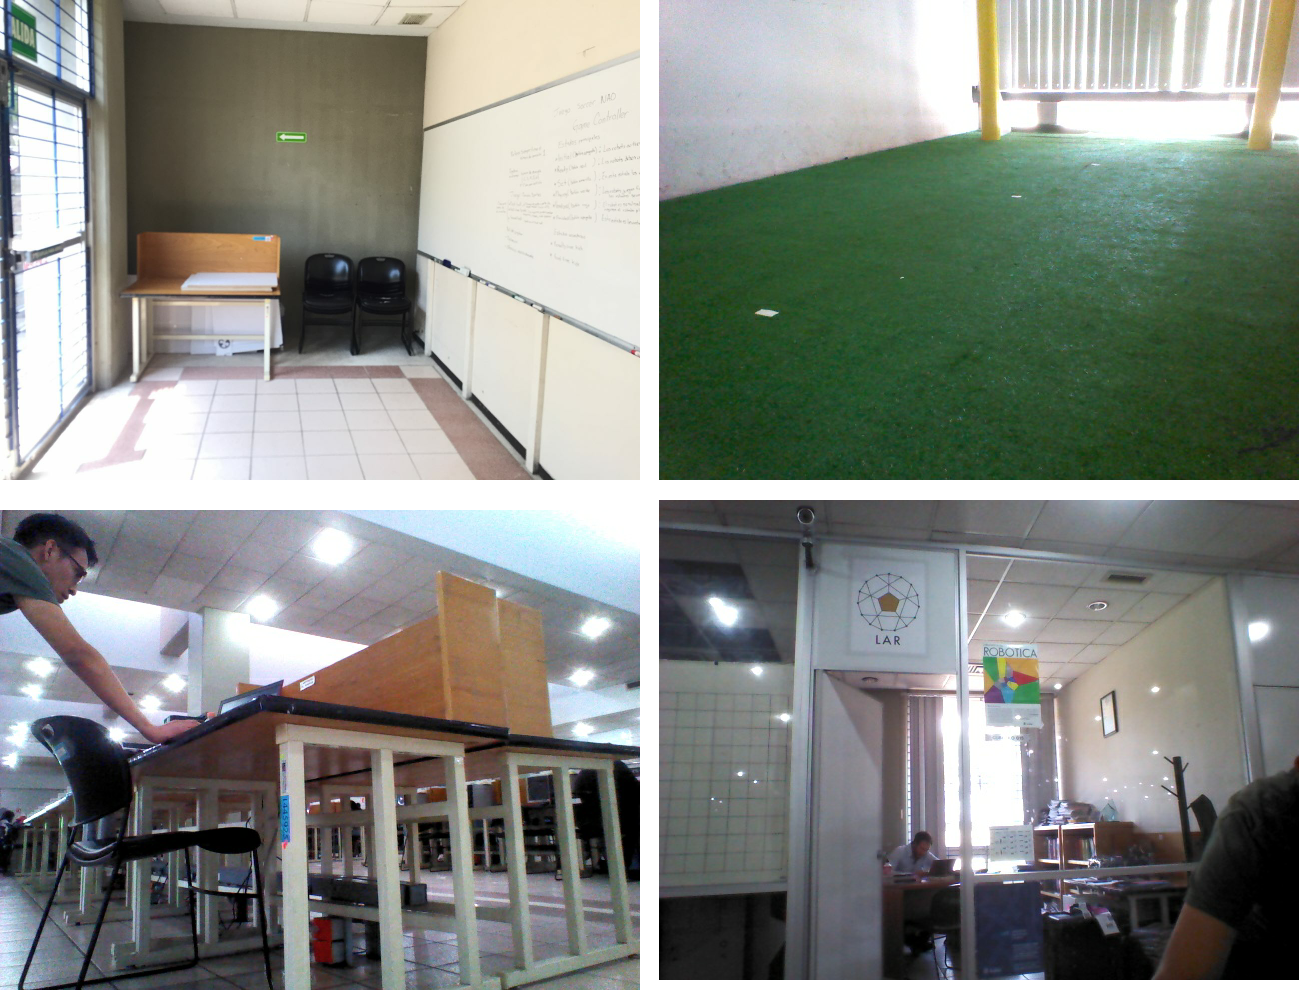
\includegraphics[width=0.5\textwidth]{scenes.png}
    \caption{Fotografías de las cuatro zonas dentro del laboratorio. De izquierda a derecha y
    de arriba a abajo: salida, cancha, zona de trabajo y cubículo.
    }
    \label{fig:scenes}
\end{figure}

Las imágenes se obtuvieron desde el robot usando el módulo de
\texttt{ALVideoRecorder},
el cual permite guardar secuencias de video utilizando las cámaras del robot y guardarlas 
en su disco. De los videos se extrajeron algunos fotogramas, no todos para evitar
redundancias, los cuales se separaron en carpetas
de acuerdo al lugar (categoría) que pertenecían. Después de este proceso
de obtención de imágenes a partir de video y de su separación en cada clase, se
generaron dos conjuntos, el de entrenamiento y el de prueba. El conjunto 
de entrenamiento está compuesto por $6000$ imágenes, $1500$ por cada clase.
El conjunto de prueba contiene $2112$ imágenes, $528$ por cada categoría.
En ambos conjuntos cada imagen es de $60 \times  80$ pixeles y de tres canales por ser imágenes en el modelo de color RGB.



\subsection{Arquitectura de la CNN}

La selección de una arquitectura para la CNN y de sus parámetros se
realizó a través de pruebas. Se tomó como base 
la arquitectura LeNet-5 (una variante de la arquitectura LeNet  que fue una de las primeras CNN que operaba sobre el 
conjunto MNIST de dígitos escritos a mano) y se probó cambiando
diversos parámetros como el número y tamaño de los kernels, la tasa de aprendizaje y el número de unidades en las capas completamente conectadas.

El primer parámetro importante son las dimensiones de
la entrada de la red. El valor de éste se mantuvo del
modelo LeNet-5 donde las imágenes tiene tamaño de $32 \times 32$,
con la adición de que las imágenes en nuestra red
tienen tres canales porque se encuentran en el espacio de 
color RGB.

\begin{figure}[!ht]
\centering
\caption{Arquitectura LeNet-5}
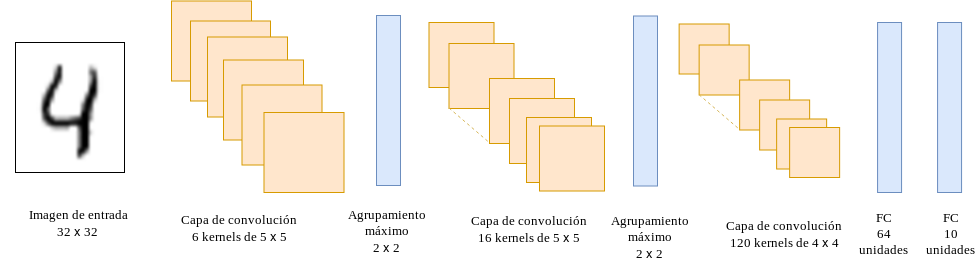
\includegraphics[scale=0.4]{lenet}
\end{figure}

LeNet-5 consiste de dos capas de convolución seguidas de dos
capas completamente conectadas, donde la última produce
la salida de la red.
Por facilidad sólo se experimentó con modelos de una y dos capas
de convolución. Las dimensiones de los kernels  que se probaron fueron de 
$7 \times 7$,
$5 \times 5$ y $3 \times 3$. En el caso de los modelos con
dos capas de covolución se pusieron por pares los tamaños de
los kernels; $7 \times 7$ con
$5 \times 5$, y $5 \times 5$ con $3 \times 3$, donde los kernels
de dimensión mayor iban en la primera capa de convolución.
Para estructuras con una capa de convolución los kernels
se mantuvieron con una dimensión de $5 \times 5$.
El número de mapas de características que se deberían producir
en cada capa de convolución se tomó de entre los valores: $8$, 
$16$, $32$, emparejando $8$ con $16$ y $16$ con $32$.
Donde $8$ y $16$ son el número de mapas obtenidos de la primera 
capa de convolución y $16$ y $32$ para la segunda.
Queremos mantener el tamaño de los mapas de
características del mismo que el de las entradas de la convolución,
esto se logra con un borde de ceros llamado \textit{same}, 
el cual se asegura que las salidas y entradas tengan las mismas dimensiones. 
La zancada o stride se mantiene constante con un valor de $1$.
Para la parte del pooling queremos ir disminuyendo las 
dimensiones de las entradas a la mitad después de cada
convolución, por lo que se ocupa un agrupamiento máximo 
de $2 \times 2$.


En cuanto a las capas completamente conectadas, se evaluaron
modelos con una capa oculta y una capa de salida y estructuras
con únicamente la capa de salida. El número de unidades 
en la capa oculta se escogió de entre los valores $1024$,
$512$ y $128$. En la capa de salida la primera unidad corresponde a la
categoría de \textit{zona de trabajo}, la segunda a 
\textit{salida de emergencia}, la tercera a \textit{cubículo}
y la última a \textit{cancha de fútbol}.

La función de activación que se utiliza en la capa de
convolución es la función ReLU. En las arquitecturas con
una capa oculta, la salida de ésta también se pasa 
por una función de activación ReLU. Para la salida 
de la red, queremos una distribución de probabilidad
sobre un conjunto de etiquetas mutuamente excluyentes.
Esto es, queremos que la salida de la unidad $i$ en la capa
de salida nos de la probabilidad $p_i$ de que una imagen que
entra
a la red pertenezca a la categoría $i$. Para nuestro caso en específico
la salida sería un vector $\mathbf{p} = (p_1, p_2, p_3, p_4)$ donde $\sum_{i = 1}^4 p_i = 1$.
El cálculo de los valores de $\mathbf{p}$  se logra usando una la función \textit{softmax}.\\

\begin{remark}

La función softmax se emplea para mapear un vector $\mathbf{z} \in \mathbb{R}^k$,  en un vector $\sigma(\mathbf{z})$ de dimensión $k$ de valores reales en el rango $(0, 1]$ cuya suma es igual a $1$. La función está dada por: 
\end{remark}

\[
\sigma : \mathbb{R}^k \rightarrow \bigg \{ \sigma \in \mathbb{R}^k | \sigma_i > 0, \sum_{i=1}^k \sigma_i = 1 \bigg \}
\]

\[
\sigma(\mathbf{z})_j = \frac{e^{z_j}}{\sum_{i=1}^k e^{z_i}} \text{ para  } j=1,\dots,k
\]
%
%donde $\hat{p}_n$ es el resultado de la unidad de cómputo antes de pasarlo
%por una función de activación, es decir, no normalizado. Es claro
%que para esta función se necesitan los valores no normalizados
%de las otras unidades en la misma capa.

El tipo de función de costo depende principalmente de la tarea a realizar,
para nosotros una tarea de clasificación en múltiples clases. La función
de costo asociada con este problema es la \textit{entropía cruzada}.\\

\begin{remark}
La entropía cruzada mide la diferencia entre dos distribuciones de probabilidad, y está
definida como sigue:

\[
L(\mathbf{y}, \mathbf{p}) = - \sum_{n} y_n log(p_n) \text{		} n \in [1,N]
\]

donde $\mathbf{y}$ denota la salida deseada y $\mathbf{p}$ contiene las probabilidades
para categoría. Si hay $N$ unidades en la capa de salida, entonces
$\mathbf{p}, \mathbf{y} \in \mathbb{R}^N$. $\mathbf{y}$ y $\mathbf{p}$ deben ser dos distribuciones de probabilidad.
\end{remark}


Por último se utiliza el algoritmo de retropropagación para
minimizar el error actualizando los pesos de los kernels y de las capas
completamente conectadas. El modo de actualización es por lotes, 
donde el tamaño de los lotes fue de elegido entre los valores 
$100$, $200$ y $300$; y
para el número de épocas entre $500$, $1000$ y $2000$.
La tasa
de aprendizaje se tomó de entre las constantes $0.001$,
$0.001$ y $0.01$.

\begin{table}[]
\centering
\caption{Resumen de los parámetros del diseño de la CNN con los que se experimentó.}
\label{table:param_cnn}
\begin{tabular}{|l|l|}
\hline
Parámetro de diseño      & Valores probados                                                                                                                            \\ \hline
Capas                    & \begin{tabular}[c]{@{}l@{}}1 convolución 1 completa                    \\1 convolución 2 completas\\ 2 convolución 1 completa\\ 2 convolución 2 completas\end{tabular} \\ \hline
\multicolumn{2}{|l|}{Capas de convolución}                                                                                                                             \\ \hline
Tamaño del kernel        & $7 \times 7$, $5 \times 5$, $3 \times 3$                                                                                                   \\ \hline
Borde de ceros                & Same                                                                                                                                        \\ \hline
Zancada                   & 1                                                                                                                                           \\ \hline
Mapas de características & 8, 16, 32                                                                                                                               \\ \hline
Pooling                  & \begin{tabular}[c]{@{}l@{}}Agrupamiento máximo (vecindades de \\ $2 \times 2$).\end{tabular}                                                \\ \hline
Función de activación    & ReLU                                                                                                                                        \\ \hline
\multicolumn{2}{|l|}{Capas completamente conectadas}                                                                                                                   \\ \hline
Salidas                  & 1024, 512, 128, 4                                                                                                                               \\ \hline
Funciones de activación  & ReLU y Softmax                                                                                                                              \\ \hline
\multicolumn{2}{|l|}{Aprendizaje}                                                                                                                                      \\ \hline
Función de costo         & Entropía cruzada                                                                                                                            \\ \hline
Optimizador              & Descenso de gradiente                                                                                                                       \\ \hline
Modo de actualización de pesos & Por lotes
\\ \hline
Tamaño del lote & 100, 200, 300
\\ \hline
Épocas & 500, 1000, 2000
\\ \hline
Tasa de aprendizaje & 0.0001, 0.001, 0.01
\\ \hline
\end{tabular}

\end{table}

A partir de estos parámetros se pueden formar $756$ arquitecturas distintas. 
La estructura de la red tiene cuatro formas posibles, dos capas de convolución
y dos completamente conectadas, dos de convolución y una completa, una de convolución
y dos completas y por último una de convolución y una completa. 

Para estructuras con dos capas de convolución y dos capas completamente conectadas 
tenemos dos
pares de dimensiones para el kernel y dos pares para el número de mapas de 
características. Podemos escoger tres valores para el número de unidades 
en la cada oculta. Y tenemos tres valores distintos para la tasa de aprendizaje, 
el número de épocas y el tamaño del lote. Por lo que tenemos un total
de $2 \times 2 \times 3 \times 3 \times 3 \times 3 = 324$ modelos posibles. 

Para los siguientes casos: dos capas de convolución y una capa completamente conectada, una capa de convolución y dos capas completamente conectadas y
una capa de convolución y una capa completamente conectada, haciendo las
mismas operaciones tenemos $108$, $243$ y $81$ respectivamente.
Un ejemplo de una de las posibles arquitecturas se muestra en la figura \ref{fig:cnn_topo_example}.

\begin{figure}[!ht]
\centering
\caption{Ejemplo de una CNN con dos capas de convolucionales y dos completamente conectadas. El tamaño de los kernels en la primera capa de convolución es de $5 \times 5$ y de la segunda de
$3 \times 3$. Los mapas de características que se obtienen de la primera y segunda capa de convolución son $8$ y $16$, respectivamente. Se utiliza un agrupamiento máximo
para reducir el tamaño de la imagen de entrada hasta un $75$ porciento. Finalmente la capa oculta conectada con la capa de salida cuenta con $1024$ unidades.\label{fig:cnn_topo_example}}
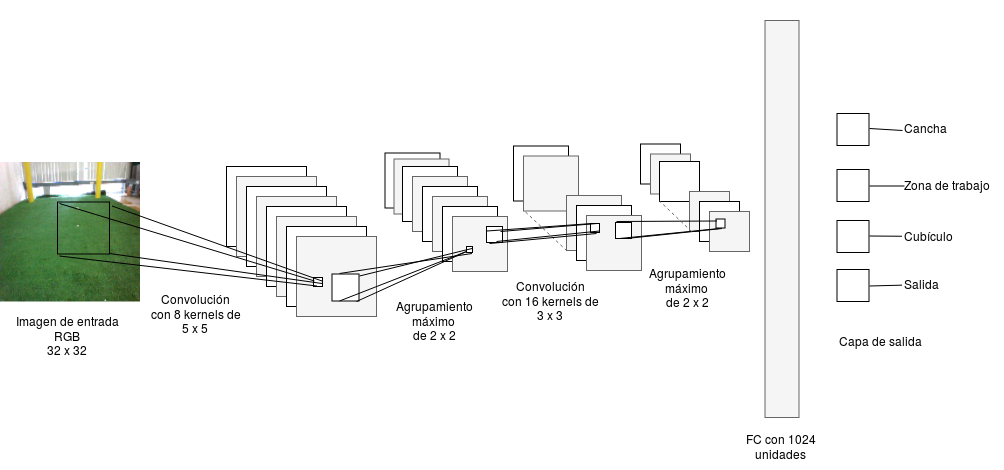
\includegraphics[scale=0.4]{cnn_topology_example}
\end{figure}
%\end{document}
